\section{Methods}\label{sec:Methods}
This section described a novel instrumentation method that leverages eye-tracking to detect in real-time which rendered objects users are looking at while working with a data visualization.  We present a general approach, details about the instrumentation of a specific data visualization, and a visual analysis system which we built to analyze eye-tracking data we collected in this way. 

\subsection{Detecting viewed objects in data visualization content}
Eye-tracking is a low resolution input. Unlike mouse input, eye-tracking can indicate a small screen region that a user is fixating, rather than a particular pixel. Typically, such a region is about one inch in diameter, though specific values depend on the user's distance to the monitor. As such, eye-tracking data cannot accurately indicate which visual object is viewed, if many objects are close together. This is not a significant problem for traditional AOI analyses, which generally use large AOIs. However, our goal was to detect the viewing of visual primitives typical of data visualization content, such as network nodes or glyphs. Generally, such visualization content is dense and intricate and eye-tracking can often not accurately discriminate between the viewing of multiple, tightly packed visualization primitives. We deal with this issue in two ways. 

First, we use a fuzzy interpretation of gaze data and detect a likelihood rather than a certainty that an object was viewed. To this end, we compute object viewing scores that range between zero- the object is not viewed, and one- the object is certainly viewed.  This is in fact a principled approach due to the eye-tracker's low resolution: sometimes there simply isn't a way to tell with absolute certainty which visual objects a user is looking at. Using a probabilistic interpretation of whether an object is viewed or not has implications on interpreting and analyzing the resulting data, which we discuss throughout the rest of the paper. Figure~\ref{fig:systemBlockDiagram} shows the concept of our system. The visualization block serves the data for the rendering to the renderer. The data is includes the position of visual objects. The renderes serves model transformation which is used to convert the stream of gaze positions from screen space to model space. The object detection algorithm collects the model space positions of visual objects from the rendered, model space positions of gazes from the screen to model transform and, the prediction scores of visual objects. The algorithm calculates the fuzzy score of visual objects which is used as an input to the object viewing prediction modules. The detail calculations of the algorithm is described later in the section.

\begin{figure}[htb]
  \centering
  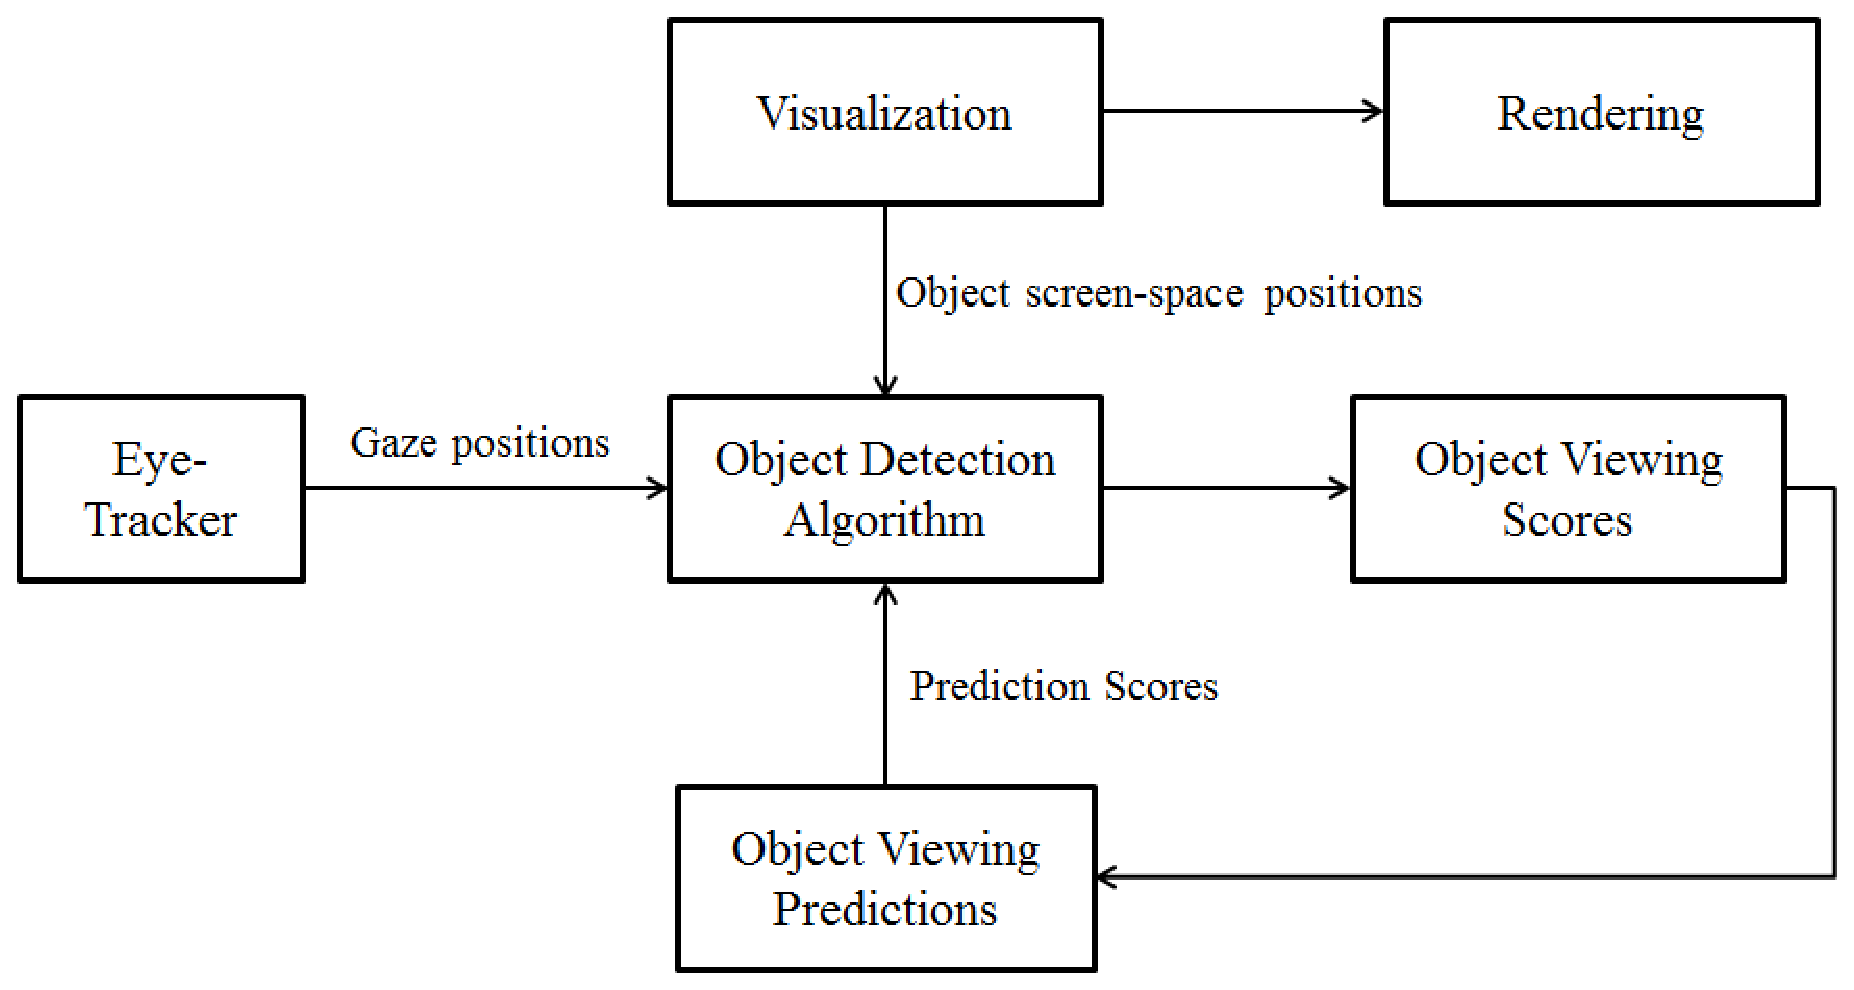
\includegraphics[width=\linewidth]{images/systemBlockDiagram.eps}
  \caption{Real-time detection of viewed objects in generative visualizations.}
	\label{fig:systemBlockDiagram}
\end{figure}

Second, analysis of eye-tracking data over interactive stimuli is a challenge. Figure~\ref{fig:AOIInteractive} shows one example of it. At time $t$ an user is looking at a view which is shown in Figure~\ref{fig:AOIInteractive}(a). The main interest of analysis is two blocks containing movie name:``Raiders of the Lost Ark'' and ``Star Wars: Episode V - The Empire Strikes Back''. The red rectangle around them shows the AOIs defined at time $t$. At time $t+1$ the user zooms out and translates the view downward which is shown in Figure~\ref{fig:AOIInteractive}(b). The AOIs drawn at time $t$ becomes inapplicable at the view of time $t+1$. At time $t+1$ a new set of AOIs need to defined. Our method automatically defines the AOIs.

\begin{figure}[htb]
  \centering
  \includegraphics[width=\linewidth]{images/AOIInteractive.eps}
  \caption{AOI analysis in interactive visualization: (a) The view at time $t$. (b) At time $t+1$, the user zooms out and translates the screen. The AOIs are automatically re-defined.}
	\label{fig:AOIInteractive}
\end{figure}

Third, we leverage Salvucci's paradigm of ``intelligent gaze interpretation''~\cite{salvucci2000intelligent} to increase the accuracy of pin-pointing which particular object is viewed when a gaze-sample is registered in the vicinity of multiple objects. We do this by predicting which of these objects is the most likely viewing target at that particular moment in time. We make such predictions based on the visualization's properties and knowledge about how the visualization is generally used. An example scenario is shown in Figure~\ref{fig:discreminate}: four visual objects ($O_{1\ldots 4}$), two of which are connected ($O_1$ and $O_3$), and one of which is highlighted ($O_3$), are shown on the screen. A gaze sample registers between $O_3$ and $O_4$. Intuitively, it is more likely that $O_3$ was viewed since it is highlighted. Moreover, if we knew that $O_1$ was viewed just before the current moment, this assumption becomes stronger, since users are more likely to look at connected elements together. 

\begin{figure}[htb]
  \centering
  \includegraphics[width=\linewidth]{images/discreminate.eps}
  \caption{``Intelligent gaze interpretation'' is used to pin-point which object is most likely to be viewed, when gazes fall in the proximity of multiple objects ($O_3$ and $O_4$). Four objects $O_{1..4}$ are shown on the screen, two of which are connected ($O_1$,$O_3$), and one of which is highlighted ($O_3$). Given that at a previous moment time, $O_1$ or $O_2$ may have been viewed ($vs1 = 0.6$, $vs2=0.6$), that $O_1$ is connected to $O_3$, and that $O_3$ is highlighted, we augmented a raw gaze scores $gs$, computed from the gazes position, with  a prediction $ps$ that $O_3$ is more likely to be viewed than $O_4$.}
	\label{fig:discreminate}
\end{figure}

The long formulas shown in the middle of Figure~\ref{fig:discreminate} exemplify how we express this intuition computationally to create an ``intelligent gaze interpretation'' algorithm that is tailored to visualization content. The assumption that people often look at connected items together is quantified in the transition probability table. However, we do not know with absolute certainty that $O_1$ was viewed previously. In fact, $O_1$'s previous viewing score ($vs_1=0.6$), is just slightly larger than $O_2$'s viewing score ($vs_2=0.5$). As such, an absolute choice of $O_1$ over $O_2$ as the previously viewed element is rather arbitrary. To avoid this, we use a weighted average of transition probabilities from $O_1$ and $O_2$ to $O_3$ and $O_4$, using the previous view scores of $O_1$ and $O_2$ as weights.  The assumption that people are more likely to look at $O_3$ because it is highlighted is captured by the visual probability $VP$. The transition and visual probabilities are combined into a prediction score $ps$. We then normalize the prediction scores we obtained for $O_3$ and $O_4$ by their largest value, since we assume that at least one of the objects must be viewed if the users gazes their vicinity. Finally, we multiply these prediction scores to $O_3$ and $O_4$'s gaze scores, $gs$, a score that is strictly based on the proximity of the gaze sample to each visual object. The result is that $O_4$ will have a slightly larger overall viewing score than $O_3$, even though the gaze sample landed equidistantly from $O_3$ and $O_4$. 

Thinking of the previously viewed objects $O_1$ and $O_2$ as referees with varying degrees of influence in a competition between $O_3$ and $O_4$, provides an intuition for an additional important guideline: an object should not referee a competition that it is part of. For example, using $O_3$ as a previous element in a competition between itself and $O_4$ would result in an open feedback-loop and should be avoided. However, the visual probability can be used to discriminate between the objects regardless of such restrictions.

\begin{algorithm}
\caption{Viewed Object Detection Algorithm}
\label{alg:ObjectDetection}
\begin{algorithmic}[1]
\For{$i \gets 0 \text{ to } n-1$}
	\State $t \gets CurrentTime()$
	\State $gs(t, O_i) = 1 - \min{(1, (\frac{d}{R}))}$
	\If{$ t = 0$}
		\State $ps(t, O_i) = 1$
		\State $vs(t, O_i) = gs(t,O_i)$
	\Else
		\State $sumVST \gets 0$
		\State $sumVS \gets 0$
		\For{$j \gets 0 \text{ to } n-1$}
			\If{$vs(t-1,O_j)> 0$ and $ vs(t,O_j)> 0$}
				\State $sumVST \gets sumVST + vs(t-1, O_j) \times T(O_i,O_j)$
				\State $sumVS \gets sumVs + vs(t-1, O_j)$				
			\EndIf
		\EndFor
		\State $ps'(t, O_i) = \frac{sumVST}{sumVS} \times VP(t, O_i)$
		\State $maxPS \gets MIN\_VAL$
		\For{$k \gets 0 \text{ to } n-1$}
			\If{$gs(t,O_k)> 0$ and $ps'(t,O_k) > maxPS$}
				\State $maxPS \gets ps'(t,O_k)$
			\EndIf
		\EndFor
		\State $ps(t,O_i) = \frac{ps'(t, O_i)}{maxPS}$
		\State $vs(t, O_i) = gs(t, O_i) \times ps(t, O_i)$
	\EndIf
\EndFor
\end{algorithmic}
\end{algorithm}

We formalize the process of computing a viewing score $vs$ for object $O_i$ at time $t$  ($vs(t,O_i)$) with the following general formulas:
\begin{equation}
vs(t, O_i) = gs(t, O_i) \times ps(t, O_i)
\label{eq:VS}
\end{equation}

\begin{equation}
gs(t, O_i) = 1 - \min{(1, (\frac{d}{R}))}
\label{eq:GS}
\end{equation}

\begin{equation}
ps'(t, O_i) = \frac{\sum{vs(t-1, O_j)} \times T(O_i,O_j)}{\sum{vs(t-1, O_j)}} \times VP(t, O_i)
\label{eq:PSDash}
\end{equation}
with $O_j$ for which $vs(t-1, O_j) > 0$ and $vs(t, O_j) > 0$.

\begin{equation}
ps(t,O_i) = \frac{ps'(t, O_i)}{\max (ps'(t, O_k))}
\label{eq:PS}
\end{equation}
with $O_k$ for which $gs(t,O_k) >0$.

Two more factors need to be considered. First, to optimize for speed, we only compute prediction scores for objects with non-zero gazes. Second, we compute viewing scores for every gaze sample, rather than every fixation. We believe that doing so leads to results that are less dependent on how fixations are computed and more robust. Since our eye-tracker's sampling rate is $60$Hz, the scores $vs(t-1)$ indicate objects that were `viewed' just $15$ms ago, an interval much shorter than the time it takes for people to shift their attention to a new object. As such, instead of using the raw $vs(t-1)$ score, we use an average of the last several viewing scores. For all practical purposes, the term $vs(t-1,Oj)$ should be replaced in the previous formulas by $ \sum_{k=1}^{k=20}{vs(t-1, O_j}$. The algorithm pseudocode is provided in Algorithm~\ref{alg:ObjectDetection}.


\subsection{Instrumenting a visualization}

\begin{figure}[htb]
  \centering
  \includegraphics[width=\linewidth]{images/pivotpaths.eps}
  \caption{PivotPaths visualization of IMDB data. Movies are displayed in the center of the scree, actors at the top, and directors and genres share the bottom space. Actors, directors, and genres associated to movies are connected through curves. Users can highlight objects and connections by hovering over them.}
	\label{fig:pivotpaths}
\end{figure}
We have use the previously described principles to instrument Doerk's interactive PivotPaths visualization of multifaceted data~\cite{dork2012pivotpaths}, which we linked to the popular internet movie database (IMDB). Shown in Figure~\ref{fig:pivotpaths}, the visualization renders movies in the center of the screen, actors on top, and genres and directors at the bottom. Actors, directors, and genres are connected by curves to the movies they associate with, and are larger, and their connections more salient, if they are associated with multiple movies. Actors, genres, and directors are colored distinctively, which is particular important for genres and directors since they occupy the same visual space. Such views are created in response to users' searches for specific movies, actors, and directors, and show data that is most relevant to the search. As shown in Figure~\ref{fig:pivotpaths}, users can hover over visual elements to highlight them and their connections. Users can also click on visual elements to transition the view to one centered on the select element. Finally, users can freely zoom and pan the visualization. 

To apply the previously described instrumentation method to this visualization, we had to define visual probabilities for objects, and transition probabilities between objects. One way to do this is by making informal assumptions about how the visualization may be directing users' visual patterns, a method employed by Salvucci~\cite{salvucci2000intelligent}. For instance, transitions between connected items may occur more often. It is reasonable to assume this, both because of the visual cue of a connecting line (i.e., users want to look at connected visuals together), but also because of the underlying data relation that the connection stands for (i.e., users want to look at connected data together). Also, transitions between objects of the same type, for instance from genre to genre, may be more dominant, especially in scanning processes. Finally, we can assume that elements that are hovered or highlighted are more likely to be viewed than those that are not, again, both because of a visual imperative (i.e., the eye is attracted to highlighted elements) and a task or data cue (i.e., the user already expressed interest in the data).

A more principled way to determine typical viewing patterns and sequences in a specific visualization is to run a preliminary eye-tracking study. In our case, we were able to leverage data collected from a pilot study, in which we instrumented an initial version of our PivotPaths visualization and collected viewing scores that were computed using gaze-coordinates alone (i.e., without including prediction scores). Analyzing the resulting data by summarizing what objects were typically viewed before other objects confirmed the assumptions we made informally (Figure~\ref{fig:transitions}, top) (e.g., transitions between connected elements are between $1.5$ and $6$ times more likely than between unconnected elements). 

Based on this information, we defined the transition and viewing probabilities as shown in Figure~\ref{fig:transitions}, bottom. These transition probabilities do not match directly the observed probabilities for the following reason. First, as can be seen in Figure~\ref{fig:pivotpaths}, movies, actors, and directors and genres occupy separate spaces. As such, it is unlikely that we will need to discriminate between a movie and an actor, or between a movie and a director. As such, we only care about how these probabilities compare to each other within the actor segment, the movie segment, and the director plus genre segment. Second, while we refer to the values in Figure~\ref{fig:transitions} as probabilities, they don't need to add to one because of the way we compute scores. 

\begin{figure}[htb]
  \centering
  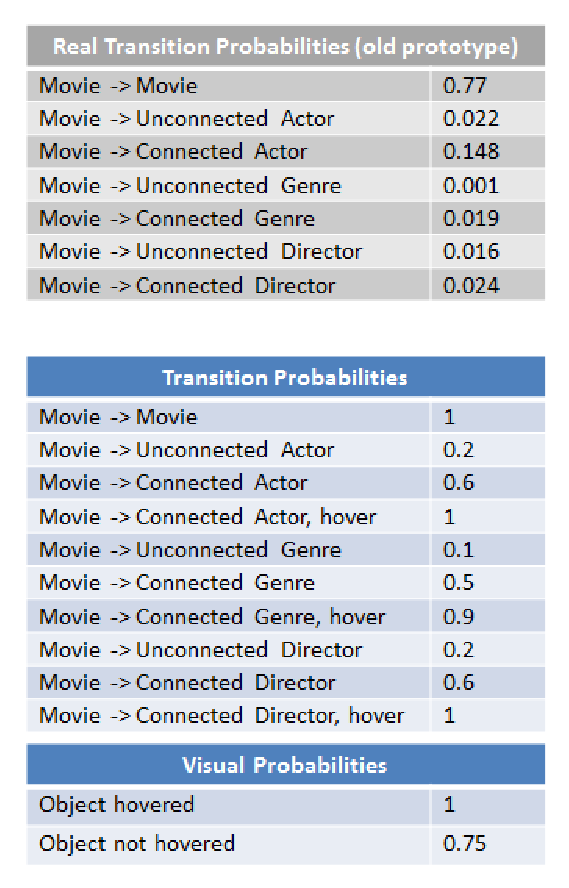
\includegraphics[width=0.75\linewidth]{images/transitions.eps}
  \caption{Transition and viewing probabilities in our instrumented visualization system (bottom two table) were informed by real patterns observed in a preliminary eye tracking study (top). }
	\label{fig:transitions}
\end{figure}

Finally, as part of instrumentation, our system collected application screen shots, mouse input events and states (e.g., cursor position, mouse press, mouse release), interactive events (e.g., hovering, zooming, panning), raw gaze samples captured at a rate of $60$Hz, and visual elements with non-zero viewing scores also captured a rate of $60$Hz, since new viewing scores are computed for every gaze sample. For each viewed element we recorded the type (i.e., movie, actor, director, genre), its gaze score ($gs$), it's prediction score ($ps$), and the aggregated viewing score ($vs$). All recorded data was time stamped. 

\subsection{Analyzing collected data}

We built a dedicated visualization system to analyze the data that our instrumentation allowed us to collect (Figure~\ref{fig:system}). We note that our main goal was to test the validity and effectiveness of capturing eye-tracking data in visualization and data space, rather than to explore generalizable and efficient techniques of analyzing such data.  

\begin{figure}[htb]
  \centering
  \includegraphics[width=\linewidth]{images/system.eps}
  \caption{A visualization system allowed to explore eye-tracking data in visualization space. A heatmap visualization at the bottom summarized which objects were viewed (left, vertically) over time (top, horizontally). Analysis could be restricted to a temporal interval by dragging start and end time lines (green and pink vertical lines). A particular moment in time could be selected (grey vertical time line) for which a screen shot of the user's activity was displayed, along with where they were looking at that time (red dot). }
	\label{fig:system}
\end{figure}

We show object viewing activity over time using a heatmap representation, by discretizing time and displaying it horizontally, and listing viewed objects vertically. The time intervals used for discretization, and the pixel size of heatmap cell could be changed interactively, thus allowing us to explore the data at multiple levels of temporal granularity. The viewed objects listed vertically were colored based on their type (movie, actor, director, genre) and could be sorted based on either first time they were viewed, amount of viewing activity, or type. 

Showing viewing data at multiple time scales requires a method of aggregating viewing scores collected every $15$ms into larger time intervals. While it may be interesting to explore the effects of different aggregation strategies, our current system only implemented one. We use Formula~\ref{eq:Aggregate} to compute the aggregated score of $O_i$ in time interval $T$. Intuitively, the formula averages all non-zero viewing scores collected in interval $T$, but also takes into account the duration of $T$. For instance, six high viewing scores recorded in a $100$ms time span are sufficient to yield a high aggregated score for that interval ( $\frac{100 \times 60 }{1000} = 6$), while for a $1000$ms interval we would require $60$ high viewing scores ( $\frac{1000 \times 60 }{1000} = 60$).
\begin{equation}
aggScore(T,O_i) = \frac{\displaystyle\sum_{t \in T }{vs(t, O_i)}}{\max (count(vs(t, O_i) > 0 , t \in T),|T| \times \frac{60}{1000}) }
\label{eq:Aggregate}
\end{equation}

The heatmap could be cleaned by filtering cells and rows. Cells could be filtered based on their value relative to the average value of all non-zero cells in the heatmap; the values of filtered cells were set to zero. Similarly, a row could be filtered depending on how its average value across all time intervals compared to such averages of other rows. Filtered rows were not shown in the heatmap. 

The system also allowed us to select a specific temporal subset of all collected data that the heatmap should display, by interactively dragging two vertical bars indicating the start and end time of the desired temporal interval. Once such an interval was defined or changed, the heatmap was recomputed to only include visual objects that were viewed in that interval. Restricting the time interval that the heatmap depicted was also reflected in filtering operations. As such, the heatmap could be configured to show objects most viewed in a temporal subset of the data, which could differ from objects most viewed in the data set as a whole.

We show interaction data as additional horizontal bars on top of the heatmap visualization. Figure~\ref{fig:system} exemplifies this: the black and grey strip indicate a change in view (e.g., new search for an actor), the pink strip indicates hovering events, and the blue strip indicates zooming or panning. 

The system allowed us to select a specific moment in time by dragging a vertical bar across the width of the heatmap. Selecting a moment in time would display a screen shot of what the user was viewing at that time, overlaid with gaze samples closest to that time point. 

Finally, the system allowed us to load data from multiple users at the same time and display views of either users' individual data, or users' aggregated data. However, aggregated user results were only computed and shown for viewing activity, by averaging user heatmaps over time. Seeing screen-shots was also disabled in aggregated mode.